\begin{figure}[H]
	\begin{center}
		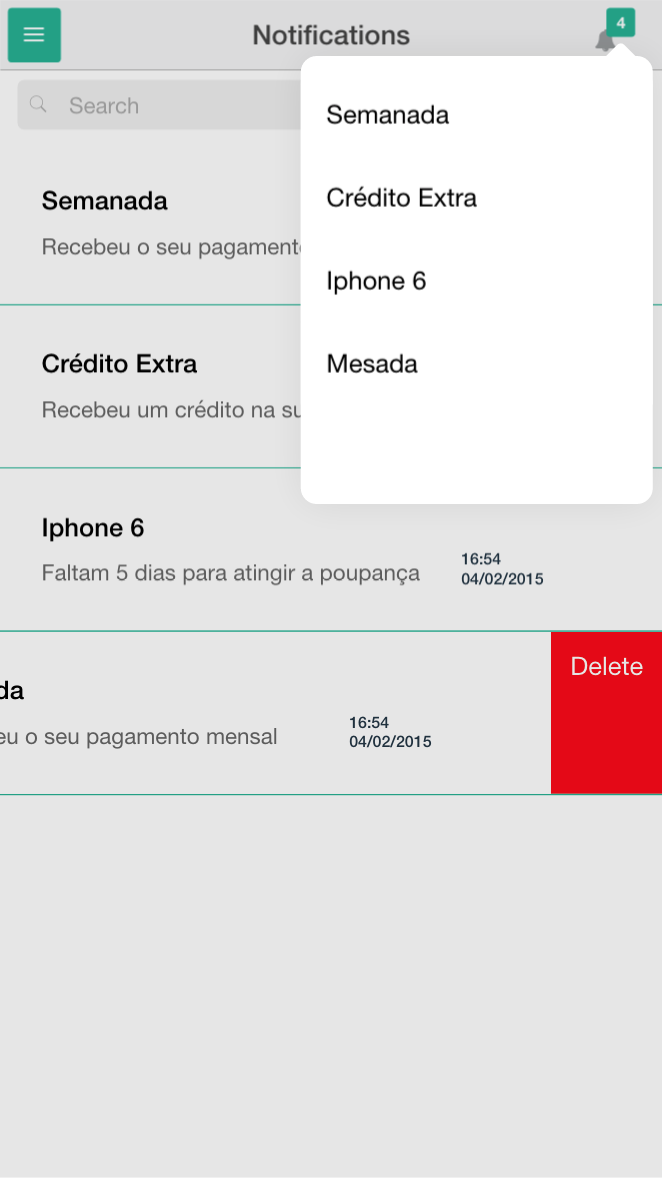
\includegraphics[width=0.5
		\textwidth]{notifications/notifications_widget.png}
	\end{center}
	\caption{\textit{Widget} de Notificações}
	\label{fig:6}
\end{figure}

É possível consultar as notificações mais recentes do utilizador selecionando o botão do canto superior direito presente em todos os ecrãs (ver Figura \ref{fig:6}).

\begin{figure}[H]
	\begin{center}
		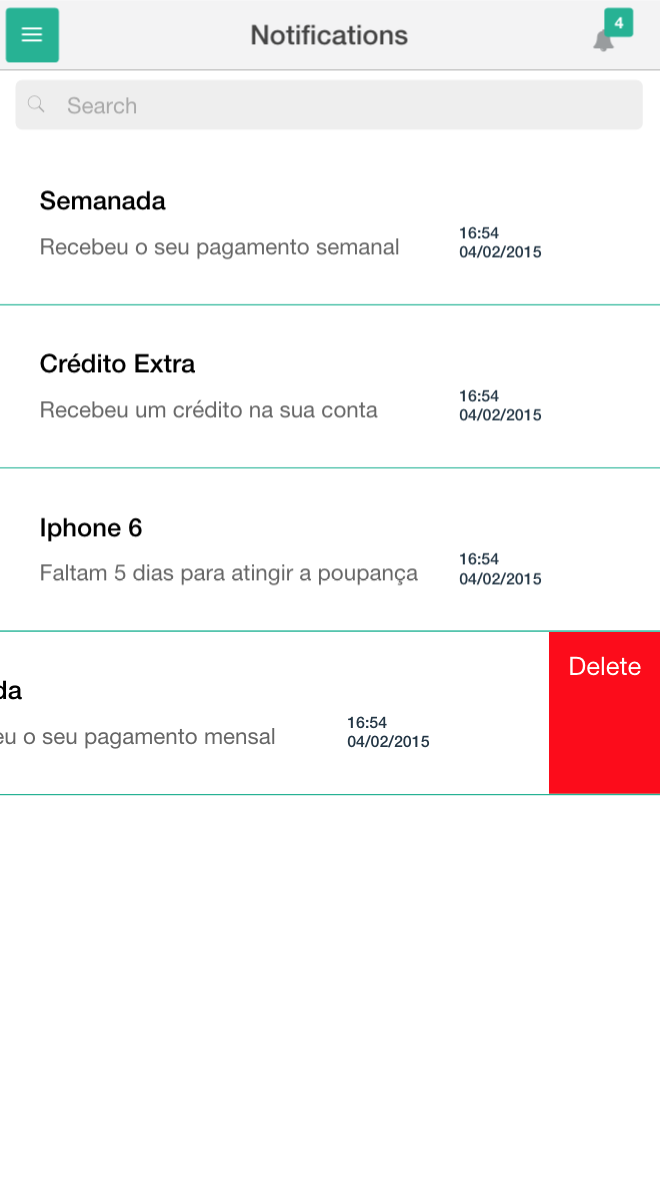
\includegraphics[width=0.5
		\textwidth]{notifications/notifications.png}
	\end{center}
	\caption{Detalhe das Notificações}
	\label{fig:6_1}
\end{figure}

É possível ver o detalhe e eliminar as notificações no ecrã de notificações acessível através do menu (ver Figura \ref{fig:6_1}).